\chapter{Multi-Modal Simulation}
\label{ch:multimodalsim}
% ##################################################################################################################

\hfill \textbf{Authors:} Christoph Dobler, Gregor Lämmel

\begin{center} 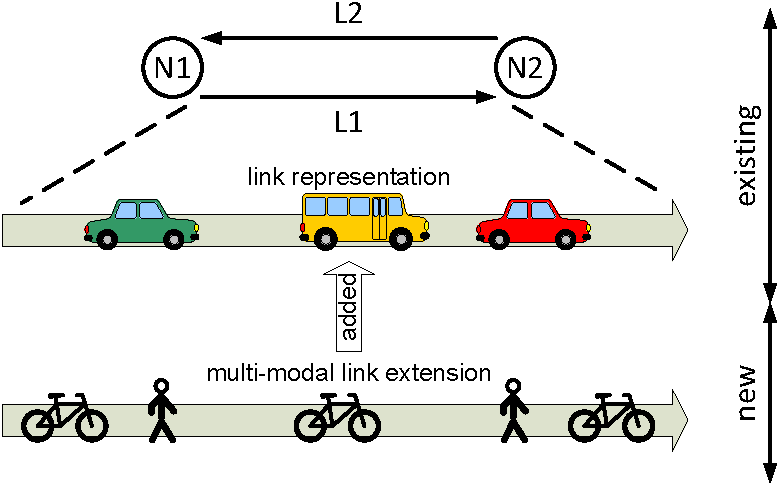
\includegraphics[width=0.5\textwidth, angle=0]{extending/figures/MultiModalSimulation/multi-modal-link-extension} \end{center}

\createStandardInformation{multimodal}{todo}{todo}{\citet{DoblerLaemmel_PED_2012}}

% ##################################################################################################################

\textit{Parts of this chapter are based on work published at the 6th International Conference on Pedestrian and Evacuation Dynamics in Zürich  \citep{DoblerLaemmel_PED_2012}}.

% ##################################################################################################################
\section{Introduction}
Having a look at today's agent-based transport simulations shows that there are two basic types of simulation models available. The first type has been developed for large-scale scenarios with hundreds of thousands or even several million entities. To keep their computational effort acceptable, they are based on simplified physical representations of traffic flows as they are known from the field of dynamic traffic assignment. In contrast, the second type of model offers a high level of detail and a microscopic modeling of the underlying physics for small scenarios with some hundred or a few thousand agents. While the first class only deals with vehicular traffic, the second one usually also deals with pedestrians and cyclists.

An approach to reduce the gap between these two simulation types is presented in the following. The proposed multi-modal simulation model adds support for ride trips and non-motorized (i.e.,\,walk and bike) traffic to a framework for large-scale simulations. The next section discusses the requirements of these multi-modal extensions. Afterward, the modeling approaches for non-motorized and ride trips as well as their implementation in \gls{matsim} are described.
%Finally, the implementations are tested by conducting experiments with a sample scenario.

% ##################################################################################################################
\section{Requirements}
Common micro-simulations focusing on vehicular traffic do not provide detailed information about the agents' positions when walking or biking. They either totally ignore non-motorized trips or \gls{teleport} agents from origins to destinations of their trips. When using the latter approach, as \gls{matsim} does so far, travel times are often determined using simple estimation rules, e.g.,\,using an average travel speed and an estimated traveled distance based on the trip's crow-fly distance.

An application's required level of detail highly influences the selection of the modeling approach. A simple model which respects agents' age and gender but does not incorporate agent-agent interactions might be detailed enough for some studies (e.g.,\,e-bikes or public transport). However, for some other studies a more detailed model, which also simulates agent interactions might be necessary (e.g.,\,evacuation of crowded pedestrian areas).

A model's computational effort increases with its level of detail. Therefore, to keep computation times short, a model should only be as detailed as necessary. On one hand, this can be realized by providing several models with various levels of detail and selecting an appropriate one. On the other hand, a flexible model with an adaptive level of detail can be used. While the latter ones are more complex, they can in turn be more detailed where needed and more aggregated where possible.

One of very few implementations of a model with different levels of detail is presented by \citet{SewallJEtAl_ACMTG_2011}. They use a hybrid model of both continuum and agent-based methods for vehicular traffic simulations. In regions of interest, the simulation uses an agent-based approach, in the remaining parts a faster continuum model.

For some applications, it is necessary that agents using different transport modes can interact. When modeling such interactions it is in general meaningful that infrastructure which would be shared in the real world is also shared in the simulation. Doing so simplifies keeping the simulation's behavior consistent. An example is the simulation of shared trips. When sharing infrastructure, an agent which performs a ride trip physically enters a vehicle and reduces its free capacity. Therefore, the agent has to wait until the vehicle has arrived and then check whether it has free capacity left. Moreover, the vehicle can wait at the meeting point if the agent to be picked up has not yet arrived.

When not sharing infrastructure, the simulation module for ride trips has to observe all vehicles and track their passengers and capacities. However, a vehicle will not recognize when a passenger has not yet arrived because it does not communicate with the ride simulation module. As a result, the vehicle will depart and the passenger will not be able to perform its scheduled ride trip. An advantage of this approach is that a ride simulation module could be developed without changing code in the vehicular simulation module.

Compared to vehicular traffic flow simulations, non-vehicular simulations require different input data. An agent's age and gender, for example, highly influences its walk speed, but is not taken into account by models for vehicular traffic flows. Models which include agent-agent or agent-environment interactions additionally need detailed information related to the road network's geometry (e.g.,\,shape, width and height profile of links) as well as buildings and other obstacles in the simulated area.

% ##################################################################################################################
\section{Modelling Approach and Implementation}
\subsection{Multi-modal Link Extension} 
\label{sec:Multi-modalSimulation}
For the simulation of non-motorized trips a new simulation module has been developed for \gls{matsim}'s \emph{QSim}. Figure~\ref{fig:multi-modal-link-extension} shows the implementation's basic concept---a multi-modal extension is added to each link object in the mobility simulation. The existing network infrastructure is re-used, which---as discussed before---simplifies the realization of interactions between agents using different transport modes.

%---------------------------------------------------------------------
\createfigure%
{Multi-modal link extension}%
{Multi-modal link extension}%
{\label{fig:multi-modal-link-extension}}%
{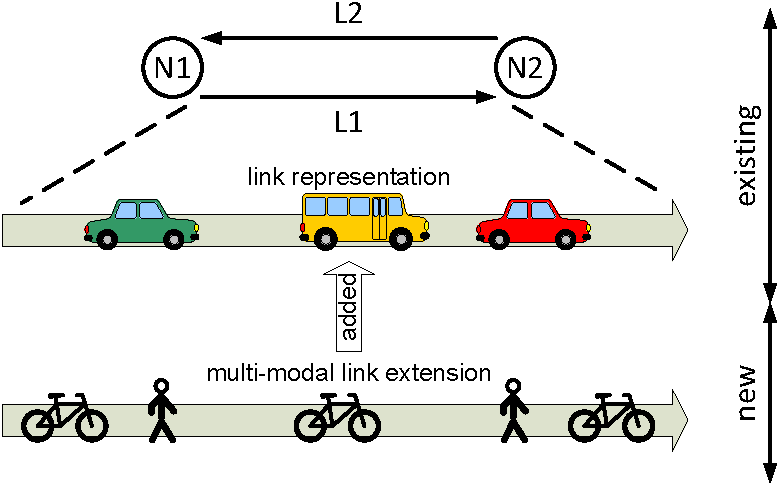
\includegraphics[width=0.75\textwidth, angle=0]{extending/figures/MultiModalSimulation/multi-modal-link-extension}}%
{}
%---------------------------------------------------------------------

While traffic flow dynamics are simulated by \gls{matsim}'s mobility simulation using a queue model, they are not taken into account in the multi-modal extension. Having a look at typical pedestrian and cyclist traffic flows shows that congestion is very rare compared to vehicular traffic and therefore justifies the application of this simplistic approach in large parts of a scenario. For regions with higher traffic flows, this simple model looses accuracy but still outperforms the teleportation approach which \gls{matsim} uses by default.

Each multi-modal link extension uses a priority queue to manage all agents traveling on that link using a non-motorized mode. The queue orders the agents based on their scheduled link leave time (see Figure \ref{fig:linkRepresentationSimpleModel}). This time is calculated when an agent enters a link based on parameters like the agent's age and gender as well as the links steepness. In each time step it is checked, whether the queue contains agents who have reached their link leave time and therefore have to be moved to their route's next link. An agent's position on a link is not determined by the model. However, under the assumption that agents move with constant speed, their position can be interpolated. This approach is computationally very efficient because computation effort is only created when an agent enters or leaves a link but not when the agent is traveling along a link. Additionally, agents can travel with different speeds and therefore overtake each other.

%---------------------------------------------------------------------
\createfigure%
{Link representation in the simple model}%
{Link representation in the simple model. \\At time 12\,084\,seconds from midnight, agent~512 enters the link and is---based on its calculated link leave time 14\,618\,seconds from midnight---inserted into the queue. At time 12\,312\,seconds from midnight, agent~780 has reached its leave time and therefore is removed from the queue.}%
{\label{fig:linkRepresentationSimpleModel}}%
{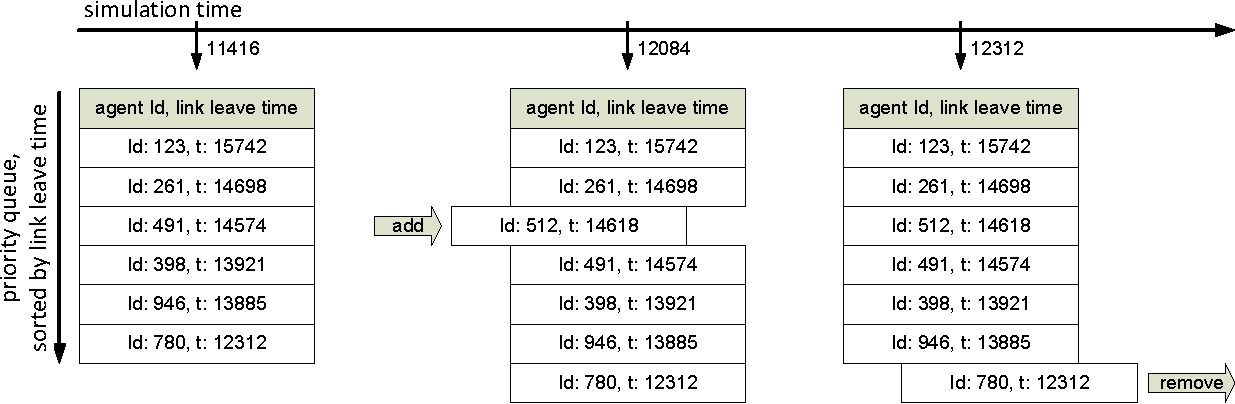
\includegraphics[width=1.0\textwidth, angle=0]{extending/figures/MultiModalSimulation/linkRepresentation}}%
{}
%---------------------------------------------------------------------

To increase the simulation's accuracy in crowded regions, models which are able to simulate interactions between agents and their environment (other agents but also other obstacles like buildings or parked vehicles) can be applied. A large group of models doing so are based on a force-based approach. There, agents' movement is based on additive attracting and repelling forces, which are ``pushing'' the agents through the environment.

In recent years, many different force-based models have been introduced and discussed. An overview is e.g.,\,given by \citet{OlesonEtAl_BazzanKluegl_2009}. Most of those models are build on the so-called social force model introduced by \citet{HelbingMolnar_PhysRevE_1995}. Collision avoiding behavior---as it can be observed in real-world situations---is implicitly reproduced by the basic social force model. It has been shown that the model works particularly well in high density conditions, such as one can observe in evacuation situations \citep{HelbingEtAl_Nature_2000}.

\citet{LaemmelPlaue_PED_2012} present an experimental implementation of a pedestrian simulation module for \gls{matsim} based on a force-base model. The agents' high-level planning (i.e.,\,route and destination choice) is performed on a graph representing the transport system (e.g.,\,a \gls{matsim} network) while the low level behavior (i.e.,\,physical interaction between the participants) is simulated with a force-based model. Besides agent-agent interactions, also interactions between agents and other obstacles are simulated. To do so, additional input data like the road network's geometry and building limits is required. Unfortunately, the scenario size is limited to a few thousand agents due to the model's high computational effort. An attempt to bypass this limitation is presented by \citet{DoblerLaemmel_PED_2012}. They combine the force-based pedestrian simulation module with the multi-modal link extension. Doing so gives the opportunity to simulate large-scale scenarios, while staying highly resolved where needed and being more aggregated where possible.

%---------------------------------------------------------------------
\subsection{Travel Times} \label{sec:TravelTimes}
Walk travel time calculation is based on results of a comprehensive literature review presented by \citet{Weidmann_TechRep_IVT_1992}. Starting point is a normally distributed reference speed of 1.34\,meters per second with a standard deviation of 0.26\,meters per second, which leads to an individual reference speed for each person. \citet{HBS_2009} and \citet{HCM_2010} report comparable but not as detailed data. If a trip's purpose is known, a person's reference value can be adjusted \citep[commuting 1.49\,meters per second, shopping 1.16\,meters per second, leisure 1.10\,meters per second; see][]{HBS_2009}. Using the reference speed and respecting a person's age, gender and statistical spreading, a personalized speed is calculated (see Figure~\ref{fig:labelPedestriansAge}). Finally, to calculate the person's travel time on a specific link, the influence of the link's steepness on the person's speed is taken into account (see Figure~\ref{fig:labelPedestriansSteepness}). The combination of person specific attributes and link steepness is shown in Figure~\ref{fig:labelPedestriansAgeSteepness3d}.

As a result, a person's speed on plain terrain is calculated as:\begin{align}
	f\textsubscript{person} = f\textsubscript{statistical~spreading} \cdot f\textsubscript{gender} \cdot f\textsubscript{age}\\
	v\textsubscript{person, walk} = v\textsubscript{reference, walk} \cdot f\textsubscript{person}
\end{align}
A link's steepness is incorporated as:
\begin{align}
    v\textsubscript{person~walks~on~link} &= v\textsubscript{person, walk} \cdot f\textsubscript{steepness}
\end{align}

%---------------------------------------------------------------------
\createfigure%
{Age and steepness dependent speed of pedestrians}%
{Age and steepness dependent speed of pedestrians}%
{\label{fig:labelWalkTravelTimes}}%
{%
  \createsubfigure%
  {Age dependent speed}%
  {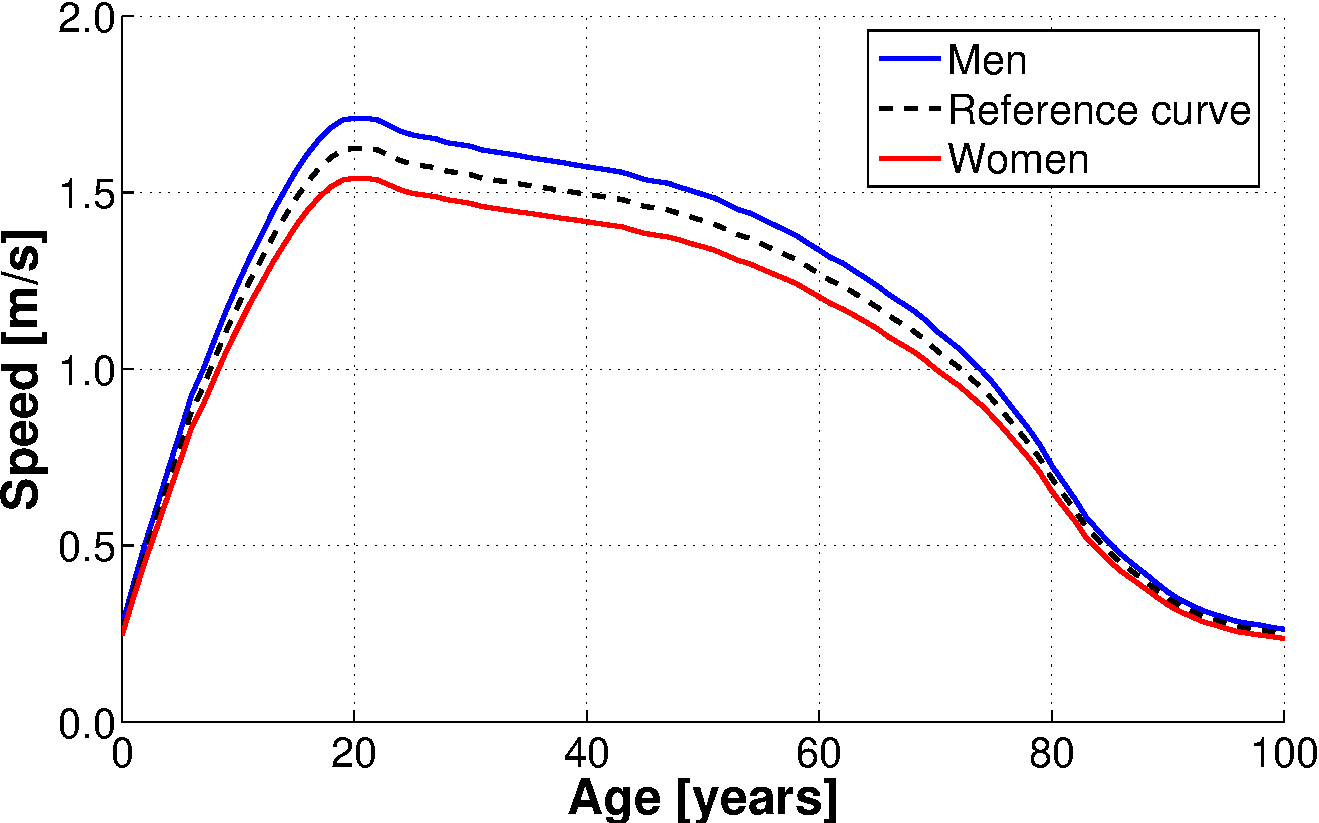
\includegraphics[width=0.65\textwidth, angle=0]{extending/figures/MultiModalSimulation/pedestriansAge}}%
  {\label{fig:labelPedestriansAge}}%
  {\vspace{3mm}}%

  \createsubfigure%
  {Steepness dependent speed}%
  {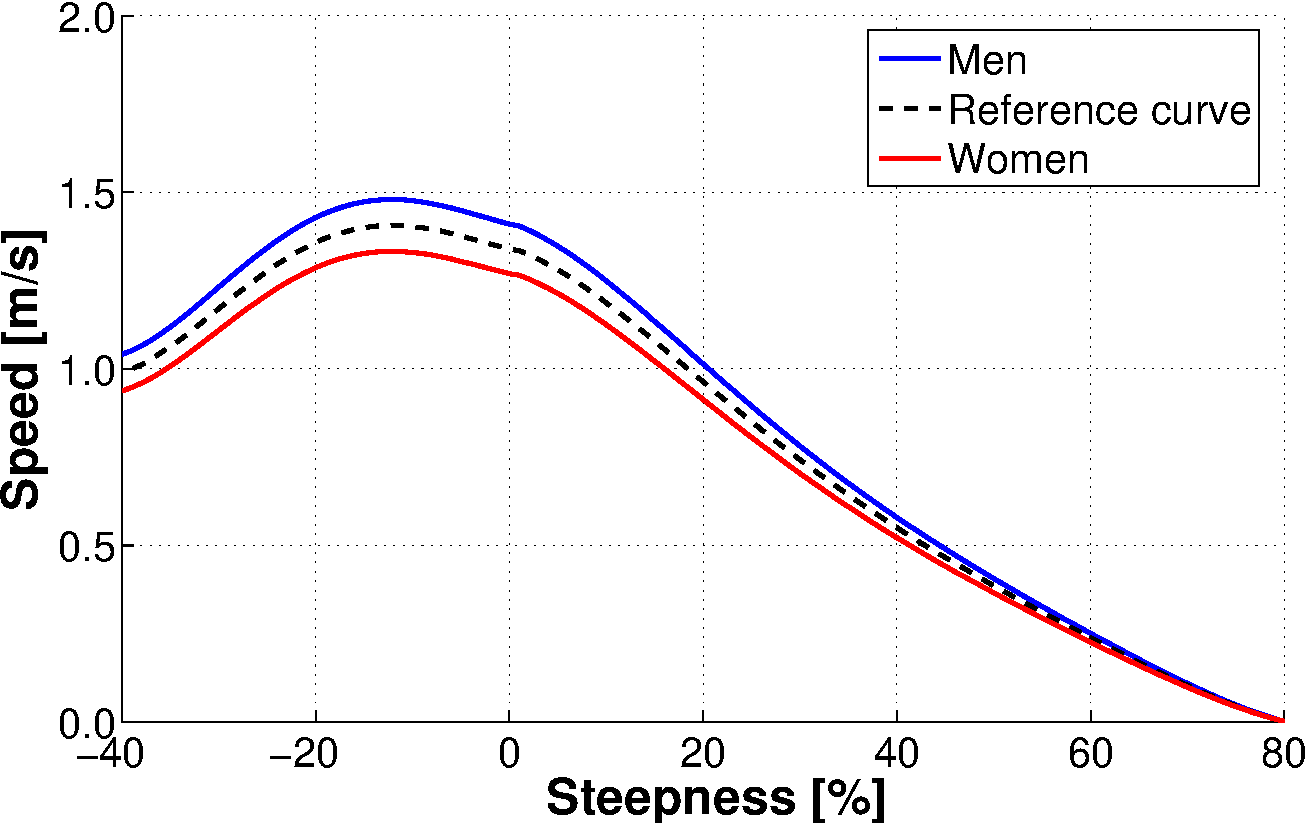
\includegraphics[width=0.65\textwidth, angle=0]{extending/figures/MultiModalSimulation/pedestriansSteepness}}%
  {\label{fig:labelPedestriansSteepness}}%
  {\vspace{3mm}}%

  \createsubfigure%
  {Age and steepness dependent speed}%
  {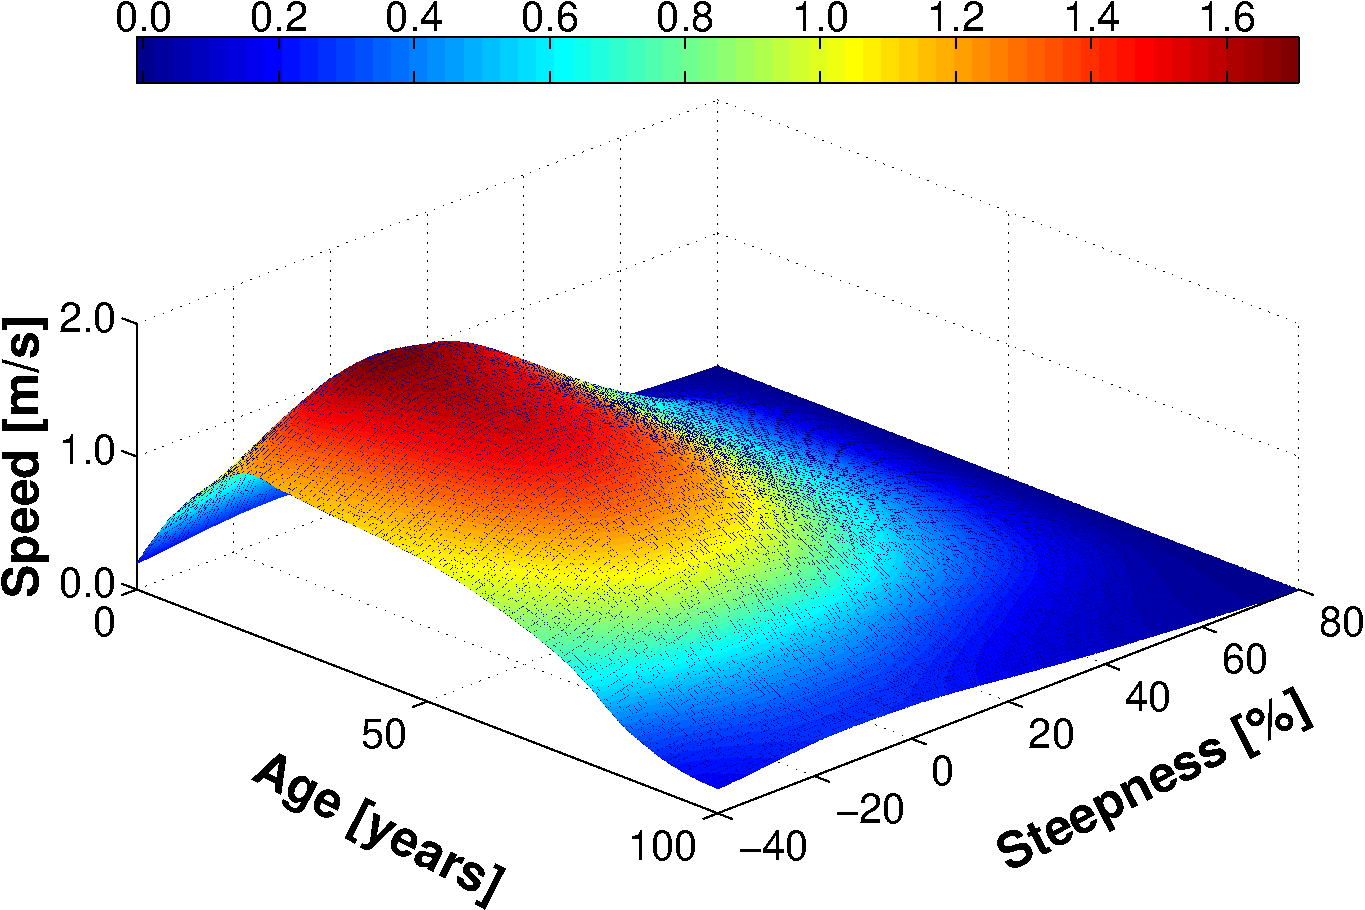
\includegraphics[width=0.65\textwidth, angle=0]{extending/figures/MultiModalSimulation/pedestrians3d}}%
  {\label{fig:labelPedestriansAgeSteepness3d}}%
  {}%
}%
{}
%---------------------------------------------------------------------

The speed of cyclists is determined using results from \citet{ParkinRotheram_TPol_2010}. Starting point is again an individual's speed based on a normal distributed ($\mathcal{N}(6.01,1.17)$) reference speed. Again, a person's speed is calculated by accounting for age and gender (see Figure~\ref{fig:labelCyclistsAge}).

%---------------------------------------------------------------------
\createfigure%
{Age and steepness dependent speed of cyclists}%
{Age and steepness dependent speed of cyclists}%
{\label{fig:labelBikeTravelTimes}}%
{%
  \createsubfigure%
  {Age dependent speed}%
  {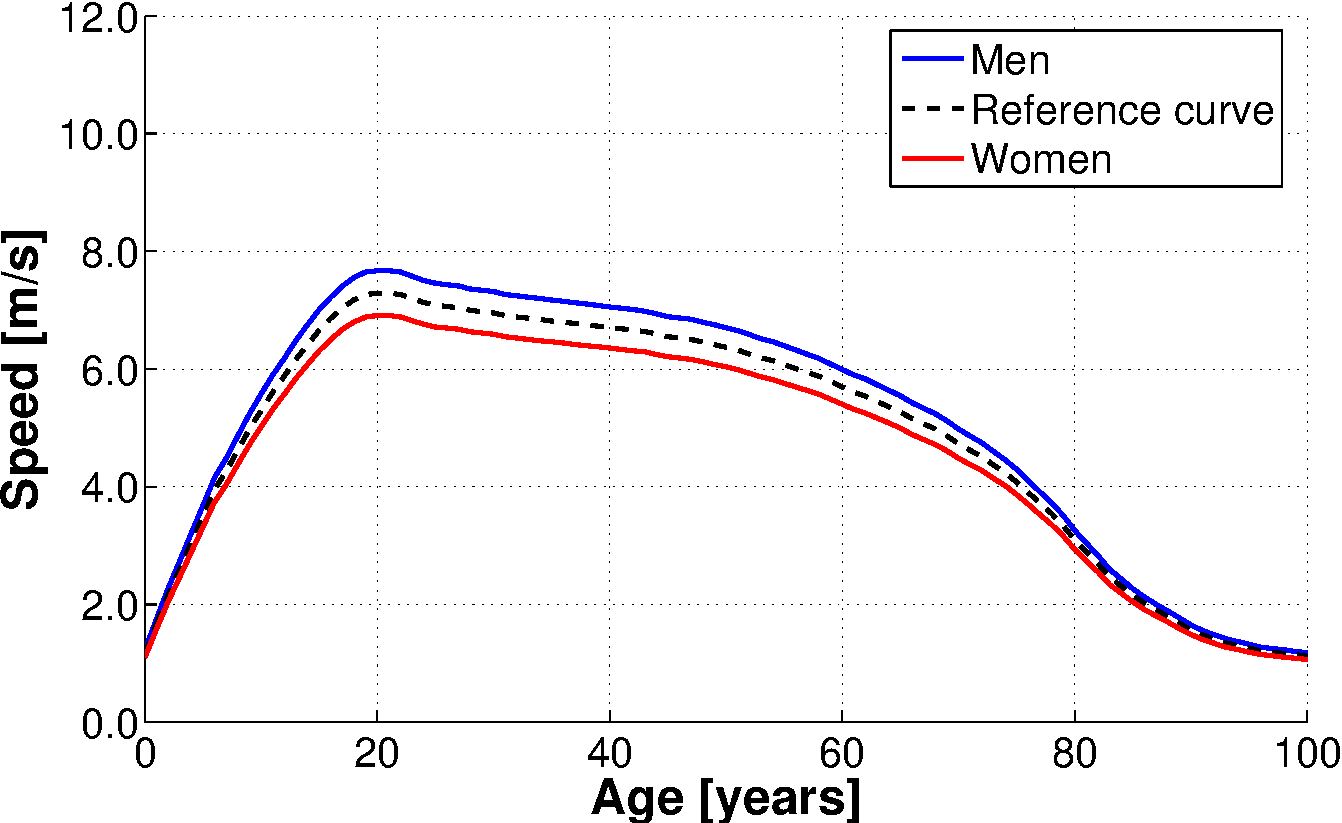
\includegraphics[width=0.65\textwidth, angle=0]{extending/figures/MultiModalSimulation/cyclistsAge}}%
  {\label{fig:labelCyclistsAge}}%
  {\vspace{5mm}}%

  \createsubfigure%
  {Steepness dependent speed}%
  {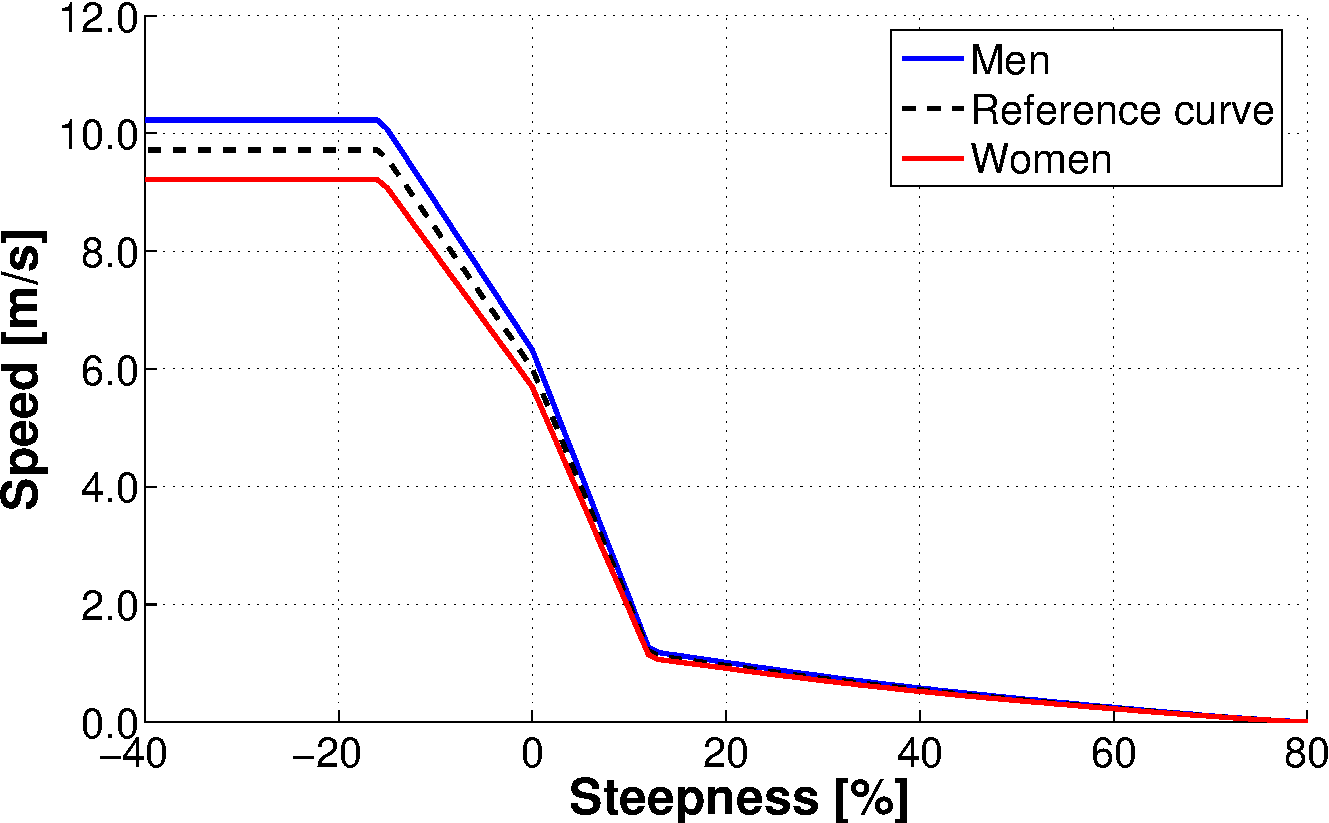
\includegraphics[width=0.65\textwidth, angle=0]{extending/figures/MultiModalSimulation/cyclistsSteepness}}%
  {\label{fig:labelCyclistsSteepness}}%
  {\vspace{4mm}}%

  \createsubfigure%
  {Age and steepness dependent speed}%
  {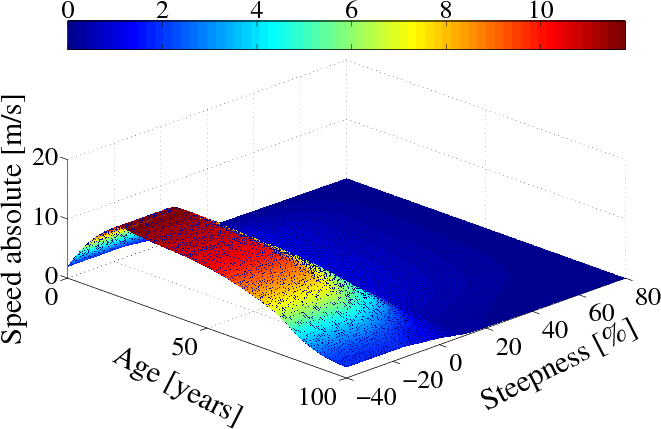
\includegraphics[width=0.65\textwidth, angle=0]{extending/figures/MultiModalSimulation/cyclists3d}}%
  {\label{fig:labelCyclistsAgeSteepness3d}}%
  {}%
}%
{}
%---------------------------------------------------------------------
\afterpage{\clearpage}	% force latex to place the figures somewhere near here and not at the end of the chapter

When calculating the steepness factor, it is distinguished whether a link goes uphill or downhill. When going uphill, the person's speed is reduced by a factor, which is calculated based on the grade and a reference factor of 0.4002\,meters per second which is scaled by the same factor as the person's reference speed. i.e.,\,the speed drop of slow people is lower than the drop of fast people. When the bike speed drops below the walk speed, which happens at a grade of approximately 12\,\%, it is assumed that the person's switches to walking (see Equation~\ref{equ:bike_uphill}). For downhill links, a reference factor of 0.2379~m/s is used. Additionally, it is assumed that cyclists limit their speed to 35\,kilometers per hour (9.7222\,meters per second; see Equation~\ref{equ:bike_downhill}).

% default seems to be ~14.0
{\fontsize{12.8pt}{12}
\begin{align}
    v\textsubscript{person, bike} &= v\textsubscript{reference, bike} \cdot f\textsubscript{person}\\
    v\textsubscript{person, uphill} &= \text{max}
    \begin{cases}
        v\textsubscript{person, bike, flat} - 0.4002 \cdot |\text{grade}| \cdot f\textsubscript{person}\\
        v\textsubscript{person, walk, uphill}
    \end{cases}\label{equ:bike_uphill}\\
    v_{\textsubscript{person, downhill}} &= \text{min}
    \begin{cases}
        v\textsubscript{person, bike, flat} + 0.2379 \cdot |\text{grade}| \cdot f\textsubscript{person}\\
        9.7222
    \end{cases}\label{equ:bike_downhill}
\end{align}
}%

Another parameter that affects the speed of pedestrians and cyclists is the crowdedness of the link where they are physically present. Data to take this effect into account is again presented by \citet{Weidmann_TechRep_IVT_1992}. However, to calculate the crowdedness of a link, its geometry has to be taken into account. A method of doing this is e.g.,\,discussed by \citet{Laemmel_PhDThesis_2011}. 

% ##################################################################################################################
\section{Conclusions}
This chapter introduced an extension of \gls{matsim}'s transport micro-simulation which adds support non-motorized trips to the framework. It allows tracking an agent's movement in detail, which is an essential requirement for studies related to topics like evacuations, e-bikes, car sharing or public transport. Experiments that test the implementation and show its capabilities are described by \citet{Dobler_PhDThesis_2013}.

A first implementation of a pedestrian simulation module for \gls{matsim} which also supports agent-agent interactions was presented by \citet{LaemmelPlaue_PED_2012}. Due to the high computational effort of the underlying physical model, the scenario size was limited to a few thousand agents. An experimental combination of their implementation and the module for non-vehicular traffic is described by \citet{DoblerLaemmel_PED_2012}. This combined implementation allowed to simulate regions of a scenario with many pedestrians with a high resolution model while other regions were simulated with the faster, but less detailed approach.

% ##################################################################################################################
